\section{Экономический раздел}
\label{sec:economy}

Данный раздел выпускной квалификационной работы предназначен для оценки оценки готовности к коммерциализации, расчёта затрат на планирование, разработку и реализацию, оценки конкурентоспособности разработанного программного решения.

\subsection{Оценка готовности к коммерциализации программной разработки <<ПК Дипломер>>}

Программный комплекс организации и выдачи верифицированных цифровых дипломов на базе блокчейна <<Дипломер>> ориентирован на выпуск и управление цифровыми дипломами в формате невзаимозаменяемых (NFT, Non-Fungible Tokens) и <<привязанных к душе>> (SBT, Soulbound Tokens) токенов.

ПК ориентирован на образовательные учреждения, академические институты, сертификационные центры, консалтинговые и коммерческие организации, предлагая средство для выпуска дипломов, сертификатов и других документов в цифровом виде с использованием технологии блокчейн, что позволяет обеспечить высокий уровень защиты данных и исключить возможность фальсификации документов. Подробное описание продукта представлено в таблице~\ref{tab:prod_spec}.

\begin{table}[H]
    \caption{Описание ниши и спецификации программного продукта}
    \centering

    \tolerance=0
    \emergencystretch=10pt
    \hyphenpenalty=0
    \exhyphenpenalty=0
    \begin{tabular}{x{8cm}x{6cm}}
        \toprule
        \textbf{Параметры спецификации}                    & \textbf{Описание} \\ \midrule
        Наименование ПО & ПК Дипломер \\
        Область применения & Образовательные учреждения, академические институты, сертификационные центры, консалтиноговые и коммерческие организации \\
        Класс программного продукта & Прикладное ПО 05.10; 12.15; 12.17 \\
        Качественные параметры получаемых результатов в процессе & Улучшения представления данных дипломов. Цифровизация документов. Защита персональных данных. \\
		Требуемый объем программных средств & Серверное приложение, смарт-контракт, клиентское приложение \\
        Сложность разработки, степень использования стандартных модулей, типовых программ & Разработка собственных решений и интеграция типовых модулей \\
        Трудоемкость разработки ПП & 1.84 \\
        Предполагаемое время разработки & 1 год \\
        Предполагаемая цена & 3.000.000 рублей \\ \bottomrule
    \end{tabular}
    \label{tab:prod_spec}
\end{table}

Из таблицы видны, что требуемый объем и состав программных средств для управления цифровыми дипломами и сертификатами через блокчейн включает серверное приложение для подготовки и формирования данных, смарт-контракт в децентрализованной сети блокчейна, клиентские приложения для запроса и просмотра дипломов.

Продукт относится к классам прикладного программного обеспечения (05.10) и отраслевого прикладного программного обеспечения (12.15, 12.17)~\cite{bib:reestrpo}. Решение совместимо с ЭВМ на базе процессоров с архитектурой AMD, ARM (32/64 bit) и операционными системами Windows 7, OS X 10.9 Mavericks, Linux 3.16 (в том числе Astra и Alt), Android 9 и новее.

Сложность разработки продукта --- средняя, включает разработку собственных решений и интеграцию типовых модулей. Возможно применение стандартных и проверенных технологий для обеспечения стабильности работы и безопасности данных. Предполагаемое время разработки --- 720 часов, а стоимость порядка 3.000.000 рублей, включая расходы на разработку, тестирование, доработку и поддержку ПП.

Для определения уровня готовности к коммерческому использованию авторской разработки была проведена экспертная оценка, результаты которой представлены в таблице~\ref{tab:prepare_mark}.

\begin{table}[H]
    \caption{Оценка готовности к коммерциализации}
    \centering

    \tolerance=0
    \emergencystretch=10pt
    \hyphenpenalty=0
    \exhyphenpenalty=0
    \begin{tabular}{@{}ll@{}}
        \toprule
        \textbf{Наименование критерия}                    & \textbf{Оценка} \\ \midrule
        Соответствие ожиданиям целевой группы & 5 \\
        Качество интерфейса & 3 \\
        Работоспособность и стабильность & 5 \\
        Полнота документации & 2 \\
        Комплексная безопасность & 4 \\
        Ожидаемый эффект от внедрения & 5 \\
        Известность бренда производителя & 3 \\
        Качество сервиса и обслуживания & 5 \\ \midrule
        Коэффициент степени готовности к коммерциализации & 0,8 \\ \bottomrule
    \end{tabular}
    \label{tab:prepare_mark}
\end{table}

Аргументация оценки готовности к коммерциализации:
\begin{enumerate}
    \item Соответствие ожиданиям целевой группы --- 5, поскольку продукт удовлетворяет требованиям и пожеланиям целевой группы.
    \item Качество интерфейса --- 3, из-за того, что для администратора системы предназначен только интерфейс командной строки (CLI), а для пользователя разработан минималистичный интерфейс в виде кнопок и текстовых команд, интегрированный в Telegram.
    \item Работоспособность и стабильность --- 5, поскольку система взаимодействует с децентрализованными сервисами и может использовать многочисленные точки входа, в случае отказа стандартных.
    \item Полнота документации --- 3, в связи с тем, что присутствует только необходимая для регистрации продукта в реестре российского ПО документация~\cite{bib:reestrpo_docs_list}.
    \item Комплексная безопасность --- 4, персональные данные пользователей не хранятся и не публикуются в явном виде, но абсолютной безопасности не существует;
    \item Ожидаемый эффект от внедрения --- 5, потому что целевая аудитория заинтересована проектом во время проведения опроса на ранней стадии разработки и проектирования;
    \item Известность бренда производителя --- 3, поскольку это дебютный проект организации в данной сфере.
    \item Качество сервиса и обслуживания --- 5, продукт полностью автоматизирован и имеет замкнутый цикл работы.
\end{enumerate}

Таким образом, исходя из оценок в таблице~\ref{tab:prepare_mark}, программный продукт демонстрирует высокий уровень готовности к коммерциализации с коэффициентом в размере 0.8, что соответствует готовности к выходу на рынок.

$$EAF = \frac{\left(\frac{5 + 3 + 5 + 2 + 4 + 5 + 3 + 5}{8}\right) \times 2}{10} = 0.8$$

Продукт уже обладает сформированным спросом и конкурентными преимуществами, что способствует его успешной реализации в существующих рыночных условиях. Однако, для успешной коммерциализации, следует уделить внимание полноте технической документации, известности бренда и четкому позиционированию на рынке, акцентируя внимание на уникальных характеристиках и преимуществах перед аналогами. Это позволит максимизировать рыночный потенциал и обеспечить устойчивое развитие.

\subsection{Расчет совокупной стоимости владения программной разработкой <<ПК Дипломер>>}

Для оценки затрат на разработку и внедрение программного обеспечения применялась модель COCOMO II~\cite{bib:cocomoii_gen, bib:cocomoii_win}, представляющая собой алгоритм для определения стоимости создания ПО. Оценка трудозатрат и времени, необходимого для разработки, помогает планировать бюджет, определять оптимальные сроки и стоимость реализации программного продукта.

Уровни значимости~\cite[c. 22-24]{bib:scale_f}, влияющие на стоимость, были опытным путем оценены и занесены в таблицу~\ref{tab:scale_factor} и таблицу~\ref{tab:labor_factor} для фактора масштаба и трудоемкости, соответственно.

\begin{table}[H]
    \caption{Оценка трудозатрат по разработке программного обеспечения}
    \centering

    \tolerance=0
    \emergencystretch=10pt
    \hyphenpenalty=0
    \exhyphenpenalty=0
    \begin{tabular}{@{}ll@{}}
        \toprule
        \textbf{Оценка фактора масштаба (j)} & \textbf{Значение} \\
        PREC & 3.72 \\
        FLEX & 1.01 \\
        RESL & 1.41 \\
        TEAM & 1.10 \\
        PMAT & 3.12 \\
        \midrule
        SF$_j$ & 10.36 \\
        E & 1.0136 \\
        \bottomrule
    \end{tabular}
    \label{tab:scale_factor}
\end{table}

\begin{enumerate}
    \item PREC --- средний, есть опыт в применяемых технологиях и опыт разработки продуктов для рассматриваемой сферы;
    \item FLEX --- очень высокий, но имеется незначительная жесткость;
    \item RESL --- очень низкий, 90\% рисков известны;
    \item TEAM --- очень высокий, сработанность команды на хорошем уровне;
    \item PMAT --- высокий, модель зрелости возможностей на хорошем уровне (CMM Уровень 3).
\end{enumerate}

\begin{table}[H]
    \caption{Оценка фактора трудоёмкости}
    \centering

    \tolerance=0
    \emergencystretch=10pt
    \hyphenpenalty=0
    \exhyphenpenalty=0
    \begin{tabular}{@{}ll@{}}
        \toprule
        \textbf{Оценка фактора трудоемкости ($EMj$)} & \textbf{Значение} \\
        \midrule
        PERS & 1.00 \\
        PREX & 1.00 \\
        RCPX & 1.00 \\
        RUSE & 1.24 \\
        PDIF & 1.00 \\
        FCIL & 1.30 \\
        CSED & 1.14 \\
        SIZE & 2.00 \\
        \midrule
        EAF & 1.83768 \\
        PM & 10.91 \\
        \bottomrule
    \end{tabular}
    \label{tab:labor_factor}
\end{table}

\begin{enumerate}
    \item PERS --- нормальный, персонал достаточно квалифицирован для выполнения поставленных задач;
    \item PREX --- нормальный, имеется опыт в реализации подобных продуктов;
    \item RCPX --- нормальный;
    \item RUSE --- супер высокий, решение можно будет использовать повторно;
    \item PDIF --- нормальный;
    \item FCIL --- очень низкий, оборудование необходимо закупить;
    \item CSED --- низкий.
\end{enumerate}

Исходя из приведенных в таблицах~\ref{tab:scale_factor} и~\ref{tab:labor_factor} даных были получены следующие значения:
$$EAF = 1 \times 1 \times 1 \times 1.24 \times 1 \times 1.3 \times 1.14 = 1.83768$$
$$PM = 1.83768 \times 2.94  \times 2^{1.0136} = 10.91 \text{ мес./чел.}$$

Таким образом, коэффицент $PM$, равный 10.91 мес./чел. говорит о том, что данный проект может быть выполнен за 11 целых месяцев --- одним человеком или за полгода группой из двух человек ($10.91/2=5.455$).

Факторы, указанные в таблицах~\ref{tab:scale_factor} и~\ref{tab:labor_factor}, влияют на результаты расчета затрат, определяющих совокупную стоимость владения авторской разработкой, таблицы~\cref{tab:cost_work_time,tab:exp_soft_dev,tab:calc_extra_exp}. 

\begin{table}[H]
    \caption{Расчёт полной стоимости программного продукта в части трудозатрат}
    \centering

    \tolerance=0
    \emergencystretch=10pt
    \hyphenpenalty=0
    \exhyphenpenalty=0
	\begin{tabular}{x{3cm}x{2.75cm}x{2.75cm}x{2.75cm}x{2.75cm}}
		\toprule
		\textbf{Сотрудники (i)} & \textbf{Процент затрат времени на работу i-го специалиста, \%} & \textbf{Трудозатраты, количество мес. PM} & \textbf{Средний оклад, руб.} & \textbf{Приведенные затраты специалистов, руб.} \\ \midrule
		Проектирование (Проектировщик) & 35 & 3.82 & 90000 & 343598.91 \\
		Разработка (Разработчик) & 100 & 10.91 & 120000 & 1308948.23 \\
		Тестирование (Тестировщики) & 50  & 5.45 & 60000 & 327237.06 \\
		Нагрузочное тестирование (Внедрение) & 5 & 0.55 & 120000 & 65447.41 \\
		Внедрение (Внедрение) & 5 & 0.55 & 120000 & 65447.41 \\
		Техническая документация (Производство) & 5 & 0.55 & 60000 & 32723.71 \\
        \midrule
		\multicolumn{4}{l}{Итого полная стоимость ПО в части трудозатрат} & 2143402.72 \\ 
		\bottomrule
	\end{tabular}
	
	\label{tab:cost_work_time}
\end{table}

Получается, что полная стоимость программного продукта (в части трудозатрат), с полным циклом и количеством специалистов равным 6 ($i=6$), составила 2 млн. 143 тыс. 400 рублей.

Согласно методологии, оценка стоимости трудозатрат на программное обеспечение включает в себя общую сумму заработной платы с добавлением 13\% налога на доходы. Также, помимо базовой заработной платы, необходимо учесть и дополнительные расходы, которые могут быть как обязательными, так и опциональными.

\begin{table}[H]
	\caption{Оценка стоимости разработки и внедрения программного продукта}
	\centering
	
	\tolerance=0
	\emergencystretch=10pt
	\hyphenpenalty=0
	\exhyphenpenalty=0
	\begin{tabular}{x{7cm}x{3cm}x{3cm}}
		\toprule
		\textbf{Статьи калькуляции} & \textbf{Процент расходов} & \textbf{Сумма} \\ \midrule
		Полная стоимость ПО в части трудозатрат & {---} & 2143402.72 \\
		Расходы на хозяйственные и административные нужды & 20\%   & 428680.544 \\
		Премия к заработной плате & 15\%   & 321510.408 \\
		Компенсация питания сотрудников & 2\%    & 42868.0544 \\
		Взносы на социальное страхование & 7.60\% & 223171.0912 \\ \midrule
		\multicolumn{2}{l}{Полная стоимость внедрения ПО, в т.ч. НДС 0\%} & 3159632.818 \\ \bottomrule
	\end{tabular}
	
	\label{tab:exp_soft_dev}
\end{table}

При расчете финальной стоимости внедрения также требуется учесть налог на добавленную стоимость (НДС) в размере 20\% от общей суммы, но, учитывая, что программный продукт будет внесен в реестр отечественного ПО, то НДС равен 0\%. Таким образом, полная стоимость разработки и внедрения ПП составит 3 млн. 159 тыс. 633 рубля.

На основе модели TCO от Gartner~\cite{bib:tco_gartner}, при оценке капитальных затрат учитываются не только инвестиции на внедрение программного продукта, но и затраты на техническую поддержку и консультации, необходимые для адаптации системы под потребности компании. Важно также принимать во внимание расходы на обучение сотрудников и приобретение специализированного оборудования и информационного канала для стабильной работы.

Таким образом, зная начальные капитальные затраты (полная стоимость внедрения ПО) и установленный Gartner предел в 20\%, можно вычислить максимально возможную сумму, которую компания может включить в общую стоимость владения, как расходы на обучение и подготовку персонала.
$$K_{\text{пк.}} = 3159632.82 \times 20\% = 631926.57 \text{ руб.}$$

Согласно этому пропорциональному методу, предполагаемые затраты на обучение персонала оцениваются в 632 тысячи рублей.

При оценке затрат на специальное оборудование и канал связи предполагается, что исходная техническая оснащенность равна нулю. Это допущение позволяет вычислить максимально возможную сумму, необходимую для реализации предложенного программного решения.

\begin{table}[H]
	\caption{Калькуляция затрат на закупку специального оборудования или каналов связи}
	\centering
	
	\tolerance=0
	\emergencystretch=10pt
	\hyphenpenalty=0
	\exhyphenpenalty=0
	\begin{tabular}{x{5cm}x{3cm}x{3cm}x{3cm}}
		\toprule
		\textbf{Статьи калькуляции} & \textbf{Стоимость} & \textbf{Количество, шт} & \textbf{Сумма, руб} \\ \midrule
		Серверное и сетевое оборудование, СХД & 25558 & 2 & 51116 \\
        Оборудование для информационной безопасности & 27930 & 1 & 27930 \\
        Платформа виртуализации & 0 & 0 & 0 \\
        Система резервного копирования & 31062 & 2 & 62124 \\
        Интернет с подключением от нескольких провайдеров & 5999.35 & 1 & 5999.35 \\ \midrule
        \multicolumn{3}{l}{ИТОГО на закупку, (Kр), руб} & 147169.35 \\ \bottomrule
	\end{tabular}
	
	\label{tab:calc_extra_exp}
\end{table}

На основе данных в таблице~\ref{tab:calc_extra_exp}, получиается, что затраты на закупку специального оборудования или каналов связи составляют 147 тысяч 170 рублей.

Таким образом, полная стоимость владения, приведенная в таблице~\ref{tab:tco}, авторской разработкой составит 6 млн. 782 тыс. 398 рублей.

\begin{table}[H]
	\caption{Расчёт совокупной стоимости владения (ТСО), руб.}
	\centering
	
	\tolerance=0
	\emergencystretch=10pt
	\hyphenpenalty=0
	\exhyphenpenalty=0
	\begin{tabular}{x{8cm}x{4cm}}
		\toprule
		\textbf{Капитальные затраты  (CAPEX)} & \textbf{3938728.73 руб.} \\ \midrule
		Затраты на внедрение & 3159632.82 руб.\\
        Затраты на обучение персонала & 631926.57 руб.\\
        Закупка специального оборудования или каналов связи & 147169.35 руб.\\ \midrule
		\textbf{Операционные затраты  (OPEX)} & \textbf{2843669.57 руб.} \\ \midrule
		Затраты на обновление и модернизацию & 315963.28 \\
        Расходы на управление системой & 631926.56 руб.\\ \midrule
		\textbf{Совокупная стоимость владения (ТСО)} & \textbf{6782398.27 руб.} \\ \bottomrule
	\end{tabular}
	
	\label{tab:tco}
\end{table}

\subsection{Оценка конкурентоспособности программной разработки <<ПК Дипломер>>}

Готовность продукта к коммерциализации и определение стоимости авторской разработки еще не гарантирует наличие спроса на нее. Для этих целей проводится оценка конкурентоспособности.

Конкурентоспособность ПП определяется на основе его соответствия современным требованиям рынка и актуальности на момент запуска. Анализ проводится путем сравнения с аналогичными продуктами на рынке.

В качестве конкурентов были выбраны цифровые дипломы от VK NFT~\cite{bib:vk_nft_diploma} и МФТИ~\cite{bib:mipt_nft_diploma}.

VK NFT дипломы представляют собой уникальные цифровые токены, которые содержат данные о выпускнике, такие как полное имя, год выпуска, название образовательной программы и тема дипломной работы. Основная цель этих NFT --- подтверждение завершения учебной программы и получения степени. Эти дипломы невозможно передать, продать или подделать, так как они привязаны к конкретному адресу на блокчейне.

МФТИ также внедряет NFT дипломы, которые будут выпускаться в виде цифровых изображений с метаданными о выпускнике, образовательной программе и годе выпуска. Эти дипломы позволят выпускникам подтвердить свою квалификацию в онлайн-пространстве, а также защищены от подделки и фальсификации благодаря использованию блокчейн-технологий.

Итоги оценки конкурентоспособности в баллах представлены в Приложении~\ref{appendix:software_development_estimation}. В таблице~\ref{tab:competitive_indices} приведены финальные значения индексов конкурентоспособности, рассчитанные на основе функциональных возможностей разработок, субъективных пользовательских предпочтений, а также организационных и экономических критериев.

\begin{table}[H]
	\caption{Расчет итогового рейтинга конкурентоспособности}
	\centering
	
	\tolerance=0
	\emergencystretch=10pt
	\hyphenpenalty=0
	\exhyphenpenalty=0
	\begin{tabular}{x{4cm}x{2cm}x{2.8cm}x{2.8cm}x{2cm}}
		\toprule

        \textbf{Элементы цены потребления} & \multicolumn{3}{c}{\textbf{Исследуемые Программные продукты}} & \textbf{Вес критерия} \\ \cmidrule(lr){2-4}
        & \textbf{ПП} & \textbf{ПЕРВЫЙ КОНКУРЕНТ} & \textbf{ВТОРОЙ КОНКУРЕНТ} &                   \\ \midrule
		Индекс конкурентоспособности по функциональным возможностям                     & 0,97                               & 1,00                                       & 0,72                                       & 40\%                     \\
		Индекс конкурентоспособности по субъективным пользовательским предпочтениям        & 1,00                               & 1,00                                       & 0,86                                       & 15\%                    \\
		Индекс конкурентоспособности по организационным критериям           & 1,00                               & 0,51                                       & 0,83                                       & 15\%                   \\
		Индекс конкурентоспособности по цене потребления      & 0,60                               & 1,00                                       & 0,55                                       & 30\%                     \\
		\textbf{ИТОГОВОЕ ЗНАЧЕНИЕ ИНДЕКСА}              & \textbf{0,87}                    & \textbf{0,93}                            & \textbf{0,71}                             & \textbf{100\%}           \\
		\bottomrule
	\end{tabular}
	\label{tab:competitive_indices}
\end{table}

Графическое изображение конкурентоспособности, основанное на информации из таблицы \ref{tab:competitive_indices}, демонстрируется на рисунке \ref{fig:competitive}.

\begin{figure}[H]   
	\centering
	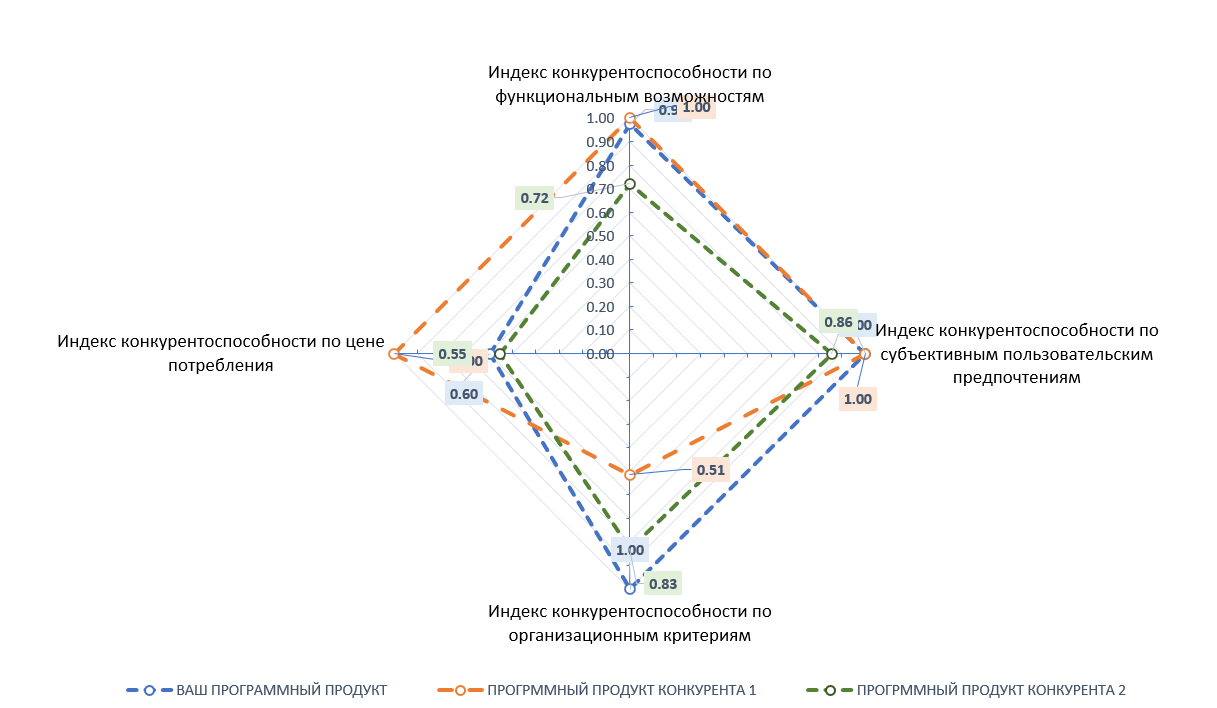
\includegraphics[width=\textwidth]{images/ec_competitive_chart.png}
	\parskip=6pt
	\caption{Радар конкурентоспособности авторской разработки}
	\label{fig:competitive}
\end{figure}

Из полученного индекса и визуализации видно, что разрабатываемый программный продукт держится среди конкурентных решений и готов к представлению на рынке. Чтобы укрепить позиуию <<ПК Дипломер>> и выбиться в лидеры, необходимо предпринять действия по улучшения отстающих параметров, которые приведены в таблице~\ref{tab:tobe}.

\begin{table}[H]
    \caption{Описание ниши и спецификации программного продукта}
    \centering

    \tolerance=0
    \emergencystretch=10pt
    \hyphenpenalty=0
    \exhyphenpenalty=0
    \begin{tabular}{x{8cm}x{6cm}}
        \toprule
        \textbf{Частные критерии конкурентоспособности} & \textbf{План действий по улучшению КП ПО} \\ \midrule
        Индекс конкурентоспособности по функциональным возможностям & Развить функциональные возможности и гибкость настрйоки приложения для обеспечения всех требуемых возможностей. \\
        Индекс конкурентоспособности по субъективным пользовательским предпочтениям & Не требуется \\
        Индекс конкурентоспособности по организационным критериям & Не требуется \\
        Индекс конкурентоспособности по цене потребления & Разработать ценовую политику и оптимизировать расходы на поддержание продукта \\ \bottomrule
    \end{tabular}
    \label{tab:tobe}
\end{table}

\subsection{Заключение по экономическому разделу}

В данном разделе была проведена комплексная оценка готовности программного решения <<ПК Дипломер>> к коммерциализации. В частности, был рассчитан коэффициент степени готовности к коммерческому применению, который составил 0.8, что свидетельствует о высокой готовности продукта к выходу на рынок.

Были оценены основные затраты на разработку, внедрение и владение программным обеспечением с использованием модели COCOMO II. Полная стоимость разработки и внедрения составила 3.159.633 рубля, а совокупная стоимость владения (ТСО) --- 6.782.398 рублей. Расчеты включали затраты на трудовые ресурсы, хозяйственные нужды, премии, компенсации, социальные взносы, а также расходы на обучение персонала и закупку специального оборудования.

Также проведен анализ конкурентоспособности продукта, включающий сравнение с аналогичными решениями от VK NFT и МФТИ. Итоговый индекс конкурентоспособности <<ПК Дипломер>> составил 0.87, что подтверждает его способность успешно конкурировать на рынке. Основные преимущества заключаются в высокой функциональности, качественном обслуживании и автоматизации процессов.

На основе проведенного анализа выявлены ключевые направления для улучшения конкурентоспособности, включая развитие функциональных возможностей приложения и оптимизацию ценовой политики. Это позволит продукту укрепить свои позиции на рынке и увеличить привлекательность для потенциальных пользователей и клиентов.

Таким образом, результаты проведенного исследования подтверждают экономическую целесообразность и рыночную перспективу коммерциализации авторского программного решения.